\documentclass[tikz,crop,convert={density=200,outext=.png},border=0.4cm]{standalone}

\usepackage{pgfplots}
\usepackage{amsmath}
\usetikzlibrary{arrows.meta}
\usepackage{physics}
\usepackage{xcolor}
\definecolor{exp_1}{RGB}{0,68,27}
\pgfplotsset{compat=newest,
    %width=6cm,
    %height=3cm,
    scale only axis=true,
    max space between ticks=25pt,
    try min ticks=5,
    every axis/.style={
        axis y line=middle,
        axis x line=middle,
        axis line style={thick,->,>=latex, shorten >=-.3cm}
    },
    every axis plot/.append style={thick},
    tick style={black, thick},
}
\tikzset{
    semithick/.style={line width=0.8pt},
}
\usepgfplotslibrary{groupplots}
\usepgfplotslibrary{dateplot}
% Document begins
\begin{document}
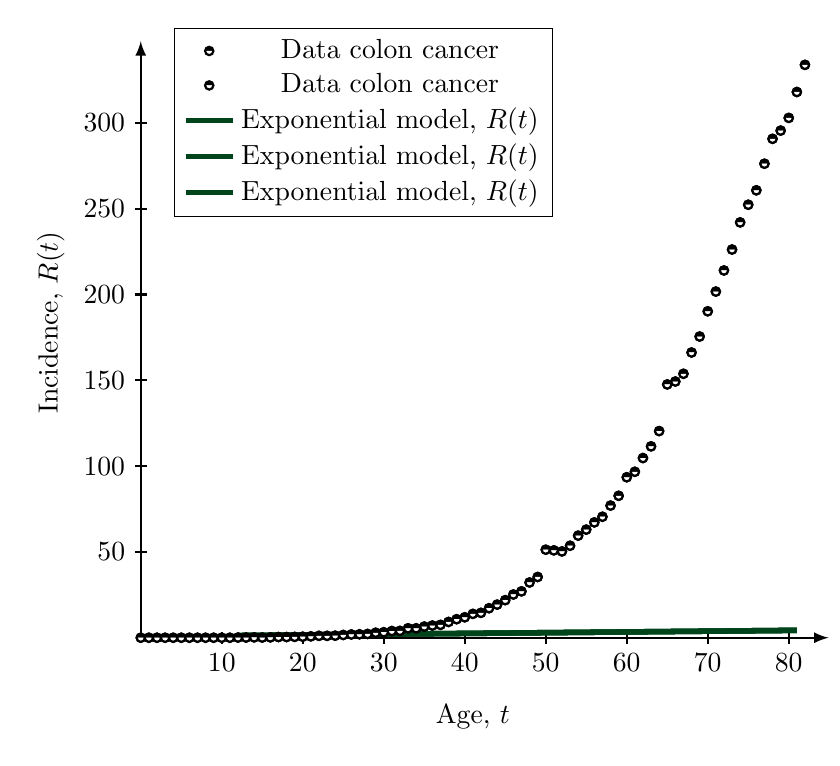
\begin{tikzpicture}
  % The axis of the plot
\begin{axis}[
    %title={Model: $\dv{y}{t}=\frac{2y}{t}$ with solution $y(t)=C_1t^2$\\Symmetry: $\Gamma_{\epsilon}=(t,y)\mapsto\left(\exp\left(\epsilon\right)t,\exp\left(-\epsilon\right)y\right)$},
    title style = {align=left},
    xlabel={Age, $t$},
    ylabel={Incidence, $R(t)$},
    x label style={at={(axis description cs:0.5,-0.1)},anchor=north},
    y label style={at={(axis description cs:-0.1,0.55)},rotate=90,anchor=south},    
    %xmin=-27, xmax=5,
    %ymin=-20, ymax=20,
    %xtick={-30,-27,...,9},
    %ytick={-15,-10,...,15},
    legend style={at={(axis description cs:0.05,0.9)},anchor=west},    
    %legend pos=north west,
    %ymajorgrids=true,
    grid style=dashed,
]
% Plot the data
\addplot[
only marks, mark=halfcircle*,mark size=1.5pt,color=black,
]
coordinates {%
(0.0,0.0)
(1.0,0.0)
(2.0,0.0)
(3.0,0.0)
(4.0,0.0)
(5.0,0.0)
(6.0,0.0)
(7.0,0.0)
(8.0,0.0)
(9.0,0.0)
(10.0,0.0)
(11.0,0.0)
(12.0,0.1)
(13.0,0.1)
(14.0,0.2)
(15.0,0.1)
(16.0,0.2)
(17.0,0.4)
(18.0,0.4)
(19.0,0.5)
(20.0,0.6)
(21.0,0.8)
(22.0,1.1)
(23.0,1.1)
(24.0,1.2)
(25.0,1.6)
(26.0,1.9)
(27.0,2.0)
(28.0,2.2)
(29.0,2.9)
(30.0,3.2)
(31.0,3.9)
(32.0,4.0)
(33.0,5.5)
(34.0,5.5)
(35.0,6.5)
(36.0,7.1)
(37.0,7.5)
(38.0,9.2)
(39.0,10.8)
(40.0,11.9)
(41.0,13.9)
(42.0,14.5)
(43.0,17.2)
(44.0,19.3)
(45.0,21.9)
(46.0,25.2)
(47.0,27.0)
(48.0,32.2)
(49.0,35.4)
(50.0,51.3)
(51.0,50.9)
(52.0,50.3)
(53.0,53.6)
(54.0,59.5)
(55.0,63.0)
(56.0,67.2)
(57.0,70.5)
(58.0,77.0)
(59.0,82.7)
(60.0,93.5)
(61.0,96.7)
(62.0,104.7)
(63.0,111.5)
(64.0,120.4)
(65.0,147.6)
(66.0,149.3)
(67.0,153.8)
(68.0,166.2)
(69.0,175.5)
(70.0,190.2)
(71.0,201.7)
(72.0,214.0)
(73.0,226.2)
(74.0,242.0)
(75.0,252.3)
(76.0,260.7)
(77.0,276.2)
(78.0,290.7)
(79.0,295.5)
(80.0,302.9)
(81.0,318.0)
(82.0,333.8)
};
\addlegendentry{Data colon cancer}
\addplot[
only marks, mark=halfcircle*,mark size=1.5pt,color=black,
]
coordinates {%
(0.0,0.0)
(1.0,0.0)
(2.0,0.0)
(3.0,0.0)
(4.0,0.0)
(5.0,0.0)
(6.0,0.0)
(7.0,0.0)
(8.0,0.0)
(9.0,0.0)
(10.0,0.0)
(11.0,0.0)
(12.0,0.1)
(13.0,0.1)
(14.0,0.2)
(15.0,0.1)
(16.0,0.2)
(17.0,0.4)
(18.0,0.4)
(19.0,0.5)
(20.0,0.6)
(21.0,0.8)
(22.0,1.1)
(23.0,1.1)
(24.0,1.2)
(25.0,1.6)
(26.0,1.9)
(27.0,2.0)
(28.0,2.2)
(29.0,2.9)
(30.0,3.2)
(31.0,3.9)
(32.0,4.0)
(33.0,5.5)
(34.0,5.5)
(35.0,6.5)
(36.0,7.1)
(37.0,7.5)
(38.0,9.2)
(39.0,10.8)
(40.0,11.9)
(41.0,13.9)
(42.0,14.5)
(43.0,17.2)
(44.0,19.3)
(45.0,21.9)
(46.0,25.2)
(47.0,27.0)
(48.0,32.2)
(49.0,35.4)
(50.0,51.3)
(51.0,50.9)
(52.0,50.3)
(53.0,53.6)
(54.0,59.5)
(55.0,63.0)
(56.0,67.2)
(57.0,70.5)
(58.0,77.0)
(59.0,82.7)
(60.0,93.5)
(61.0,96.7)
(62.0,104.7)
(63.0,111.5)
(64.0,120.4)
(65.0,147.6)
(66.0,149.3)
(67.0,153.8)
(68.0,166.2)
(69.0,175.5)
(70.0,190.2)
(71.0,201.7)
(72.0,214.0)
(73.0,226.2)
(74.0,242.0)
(75.0,252.3)
(76.0,260.7)
(77.0,276.2)
(78.0,290.7)
(79.0,295.5)
(80.0,302.9)
(81.0,318.0)
(82.0,333.8)
};
\addlegendentry{Data colon cancer}

% Plot the model
\addplot[
color=exp_1,line width=2pt,
]
coordinates {%
(12.0,1.2652772145348719)
(13.0,1.309277214534872)
(14.0,1.353277214534872)
(15.0,1.3972772145348717)
(16.0,1.4412772145348718)
(17.0,1.4852772145348718)
(18.0,1.5292772145348716)
(19.0,1.5732772145348717)
(20.0,1.6172772145348717)
(21.0,1.6612772145348718)
(22.0,1.7052772145348718)
(23.0,1.7492772145348718)
(24.0,1.7932772145348719)
(25.0,1.8372772145348717)
(26.0,1.8812772145348717)
(27.0,1.9252772145348718)
(28.0,1.9692772145348718)
(29.0,2.013277214534872)
(30.0,2.0572772145348717)
(31.0,2.1012772145348717)
(32.0,2.1452772145348717)
(33.0,2.189277214534872)
(34.0,2.233277214534872)
(35.0,2.2772772145348714)
(36.0,2.321277214534872)
(37.0,2.3652772145348715)
(38.0,2.409277214534872)
(39.0,2.4532772145348716)
(40.0,2.4972772145348716)
(41.0,2.5412772145348717)
(42.0,2.5852772145348717)
(43.0,2.6292772145348717)
(44.0,2.6732772145348718)
(45.0,2.717277214534872)
(46.0,2.761277214534872)
(47.0,2.805277214534872)
(48.0,2.849277214534872)
(49.0,2.8932772145348715)
(50.0,2.9372772145348716)
(51.0,2.9812772145348716)
(52.0,3.0252772145348716)
(53.0,3.0692772145348717)
(54.0,3.1132772145348717)
(55.0,3.1572772145348718)
(56.0,3.201277214534872)
(57.0,3.245277214534872)
(58.0,3.289277214534872)
(59.0,3.3332772145348715)
(60.0,3.3772772145348715)
(61.0,3.4212772145348715)
(62.0,3.4652772145348716)
(63.0,3.5092772145348716)
(64.0,3.5532772145348717)
(65.0,3.5972772145348717)
(66.0,3.6412772145348717)
(67.0,3.685277214534872)
(68.0,3.729277214534872)
(69.0,3.773277214534872)
(70.0,3.8172772145348715)
(71.0,3.8612772145348715)
(72.0,3.9052772145348715)
(73.0,3.9492772145348716)
(74.0,3.9932772145348716)
(75.0,4.037277214534871)
(76.0,4.081277214534872)
(77.0,4.125277214534872)
(78.0,4.169277214534872)
(79.0,4.213277214534871)
(80.0,4.257277214534872)
(81.0,4.301277214534871)
};
\addlegendentry{Exponential model, $R(t)$}
\addplot[
color=exp_1,line width=2pt,
]
coordinates {%
(12.0,1.2652772145348719)
(13.0,1.309277214534872)
(14.0,1.353277214534872)
(15.0,1.3972772145348717)
(16.0,1.4412772145348718)
(17.0,1.4852772145348718)
(18.0,1.5292772145348716)
(19.0,1.5732772145348717)
(20.0,1.6172772145348717)
(21.0,1.6612772145348718)
(22.0,1.7052772145348718)
(23.0,1.7492772145348718)
(24.0,1.7932772145348719)
(25.0,1.8372772145348717)
(26.0,1.8812772145348717)
(27.0,1.9252772145348718)
(28.0,1.9692772145348718)
(29.0,2.013277214534872)
(30.0,2.0572772145348717)
(31.0,2.1012772145348717)
(32.0,2.1452772145348717)
(33.0,2.189277214534872)
(34.0,2.233277214534872)
(35.0,2.2772772145348714)
(36.0,2.321277214534872)
(37.0,2.3652772145348715)
(38.0,2.409277214534872)
(39.0,2.4532772145348716)
(40.0,2.4972772145348716)
(41.0,2.5412772145348717)
(42.0,2.5852772145348717)
(43.0,2.6292772145348717)
(44.0,2.6732772145348718)
(45.0,2.717277214534872)
(46.0,2.761277214534872)
(47.0,2.805277214534872)
(48.0,2.849277214534872)
(49.0,2.8932772145348715)
(50.0,2.9372772145348716)
(51.0,2.9812772145348716)
(52.0,3.0252772145348716)
(53.0,3.0692772145348717)
(54.0,3.1132772145348717)
(55.0,3.1572772145348718)
(56.0,3.201277214534872)
(57.0,3.245277214534872)
(58.0,3.289277214534872)
(59.0,3.3332772145348715)
(60.0,3.3772772145348715)
(61.0,3.4212772145348715)
(62.0,3.4652772145348716)
(63.0,3.5092772145348716)
(64.0,3.5532772145348717)
(65.0,3.5972772145348717)
(66.0,3.6412772145348717)
(67.0,3.685277214534872)
(68.0,3.729277214534872)
(69.0,3.773277214534872)
(70.0,3.8172772145348715)
(71.0,3.8612772145348715)
(72.0,3.9052772145348715)
(73.0,3.9492772145348716)
(74.0,3.9932772145348716)
(75.0,4.037277214534871)
(76.0,4.081277214534872)
(77.0,4.125277214534872)
(78.0,4.169277214534872)
(79.0,4.213277214534871)
(80.0,4.257277214534872)
(81.0,4.301277214534871)
};
\addlegendentry{Exponential model, $R(t)$}
\addplot[
color=exp_1,line width=2pt,
]
coordinates {%
(12.0,1.2652772145348719)
(13.0,1.309277214534872)
(14.0,1.353277214534872)
(15.0,1.3972772145348717)
(16.0,1.4412772145348718)
(17.0,1.4852772145348718)
(18.0,1.5292772145348716)
(19.0,1.5732772145348717)
(20.0,1.6172772145348717)
(21.0,1.6612772145348718)
(22.0,1.7052772145348718)
(23.0,1.7492772145348718)
(24.0,1.7932772145348719)
(25.0,1.8372772145348717)
(26.0,1.8812772145348717)
(27.0,1.9252772145348718)
(28.0,1.9692772145348718)
(29.0,2.013277214534872)
(30.0,2.0572772145348717)
(31.0,2.1012772145348717)
(32.0,2.1452772145348717)
(33.0,2.189277214534872)
(34.0,2.233277214534872)
(35.0,2.2772772145348714)
(36.0,2.321277214534872)
(37.0,2.3652772145348715)
(38.0,2.409277214534872)
(39.0,2.4532772145348716)
(40.0,2.4972772145348716)
(41.0,2.5412772145348717)
(42.0,2.5852772145348717)
(43.0,2.6292772145348717)
(44.0,2.6732772145348718)
(45.0,2.717277214534872)
(46.0,2.761277214534872)
(47.0,2.805277214534872)
(48.0,2.849277214534872)
(49.0,2.8932772145348715)
(50.0,2.9372772145348716)
(51.0,2.9812772145348716)
(52.0,3.0252772145348716)
(53.0,3.0692772145348717)
(54.0,3.1132772145348717)
(55.0,3.1572772145348718)
(56.0,3.201277214534872)
(57.0,3.245277214534872)
(58.0,3.289277214534872)
(59.0,3.3332772145348715)
(60.0,3.3772772145348715)
(61.0,3.4212772145348715)
(62.0,3.4652772145348716)
(63.0,3.5092772145348716)
(64.0,3.5532772145348717)
(65.0,3.5972772145348717)
(66.0,3.6412772145348717)
(67.0,3.685277214534872)
(68.0,3.729277214534872)
(69.0,3.773277214534872)
(70.0,3.8172772145348715)
(71.0,3.8612772145348715)
(72.0,3.9052772145348715)
(73.0,3.9492772145348716)
(74.0,3.9932772145348716)
(75.0,4.037277214534871)
(76.0,4.081277214534872)
(77.0,4.125277214534872)
(78.0,4.169277214534872)
(79.0,4.213277214534871)
(80.0,4.257277214534872)
(81.0,4.301277214534871)
};
\addlegendentry{Exponential model, $R(t)$}

\end{axis}
\end{tikzpicture}

\end{document}
